\section{Theoretical foundations}\label{Theoretical foundations}

The following is an overview of the most important topics of significance to this research paper.

\subsection{Time series models}\label{Time series models}

In the domain of time series forecasting many models have been developed. These models can be subdivided into univariate and multivariate models. Univariate track a single variable and make predictions based on the historical values of that same variable. Multivariate track the mutual dependance of multiple variables and make predictions on there future values.

\subsubsection{Univariate}\label{Univariate}

The most important univariate models that have been developed over the years include:

\begin{itemize}
    \item \Gls{ar} \cite{whittle} - expresses the current value as a linear combination of $p$ historical values. \Glsxtrshort{ar}$(p)$ denotes an \glsxtrlong{ar} model of order $p$. The model is mathematically defined as follows:

        $X_{t} =  \varepsilon_{t} + \sum_{i=1}^{p}\phi_{i}X_{t-i}$

        where:
        \begin{itemize}
            \item $X_{t}, X_{t-i}$ are the values of the time series at time $t$ and $t-i$.
            \item $\phi_{i}$ are the coefficient for values at different time offsets.
            \item $\varepsilon_{t}$ is the random variable representing white noise.
        \end{itemize}
    \item \Gls{ma} \cite{whittle} - expresses the current value as a linear combination of $p$ historical error terms. \Glsxtrshort{ma}$(q)$ denotes an \glsxtrlong{ma} model of order $q$. The model is mathematically defined as follows:
        
        $X_{t} = \mu + \varepsilon_{t} + \sum_{i=1}^{q}\theta_{i}\varepsilon_{t-i}$
        
        where:
        \begin{itemize}
            \item $\mu$ is the the mean of the series.
            \item $X_{t}, X_{t-i}$ are the values of the time series at time $t$ and $t-i$.
            \item $\theta_{i}$ are the coefficient for error terms at different time offsets.
            \item $\varepsilon_{t-i}$ are the the white noise error terms at time $t-i$.
        \end{itemize}

    \item \Gls{arma} \cite{whittle} - combines the \gls{ar} and \gls{ma} models. \Glsxtrshort{arma}$(p)$ denotes an model with $p$ autoregressive terms and $q$ moving-average terms. \gls{arma} requires the time series to be stationary. The model is mathematically defined as follows:

        $X_{t} =  \varepsilon_{t} + \sum_{i=1}^{p}\phi_{i}X_{t-i} + \sum_{i=1}^{q}\theta_{i}\varepsilon_{t-i}$

    \item \Gls{es} \cite{brown,holt} - expresses the current value in a time series as a exponentially weighted combination of its past values where the most recent values have the most significance. Its mathematical representation is a follows:

        $S_{t} = \alpha X_{t} + (1 - \alpha)S_{t-1}$

        where:
        \begin{itemize}
            \item $S_{t}, S_{t-1}$ are the values of the smoothed time series at time $t$ and $t-1$.
            \item $\alpha$ is the smoothing factor.
            \item $X_{t}$ is the value of the time series at time $t$.
        \end{itemize}

    \item \Gls{arima} \cite{box-jenkins} - is a generalization of the \gls{arma} model which requires non-stationary series to be differenced in order for them to achieve stationarity. \gls{arima} models are denoted by: \gls{arima}$(p, d, q)$ where $p$ is the order of the \gls{ar} model, $d$ is the degree of differencing and $q$ is the order of the \gls{ma} model. Using the Box-Jenkins method allows for the selection of optimal parameters for an \gls{arima} model enabling the best fit of the model for the given time series.
    \item \Gls{rw} \cite{meese-rogoff} - is a naive model that proposes that changes between values in a time series are random and unrelated. There are two subvariants:
        \begin{itemize}
            \item \gls{rw} without drift defined as:

                $X_t = X_{t-1} + \varepsilon_t$

            \item \gls{rw} with drift defined as:
        
                $X_t = X_{t-1} + a + \varepsilon_t$

        \end{itemize}

    where:

    \begin{itemize}
            \item $X_{t}, X_{t-1}$ is the value of the time series at time $t$ and $t - 1$.
            \item $\varepsilon_t$ is the random step at time $t$.
            \item $a$ - is a constant that determines the trend of the series.
    \end{itemize}

        The \gls{rw} without drift is often used as a benchmark for various forecasting models.

    \item \Gls{arch} \cite{engle} - is a model that describes the conditional variance of a time series as an \gls{ar} combination of past squared errors. \Glsxtrshort{arch}$(p)$ denotes an \glsxtrlong{arch} model of order $p$. The time series is described by the following equation:

        $\sigma_{t}^2 = \alpha_{0} + \sum_{i=1}^{p}\alpha_{i}\varepsilon_{t-i}^2$

    where:
    \begin{itemize}
        \item $\sigma_{t}^2$ is the conditional variance.
        \item $\alpha_{0}$ is a constant term that sets the baseline level of variance.
        \item $\alpha_{i}$ are the coefficients that determine the weight of previous error terms.
        \item $\varepsilon_{t-i}$ are values of previous error terms.
    \end{itemize}

    \item \Gls{garch} \cite{bollerslev} - is an extension of \gls{arch} that allows the conditional variance to be an \gls{arma} process, rather than just an \gls{ar} process as in \gls{arch}. The \Glsxtrshort{garch}(p,q) model is described by the equation:

        $\sigma_{t}^2 = \alpha_{0} + \sum_{i=1}^{p}\alpha_{i}\varepsilon_{t-i}^2 + \sum_{j=1}^{q}\beta_{j}\sigma_{t-j}^2$

        where:
    \begin{itemize}
        \item $\sigma_{t}^2$ is the conditional variance.
        \item $\alpha_{0}$ is a constant term that sets the baseline level of variance.
        \item $p$ is the order of the \gls{ar} term.
        \item $q$ is the order of the \gls{ma} term.
        \item $\alpha_{i}$ are the coefficients of the \gls{ar} terms.
        \item $\beta_{j}$  are the coefficients of the \gls{ma} terms.
        \item $\varepsilon_{t-i}$ are values of previous error terms.
        \item $\sigma_{t-j}$ are the lagged conditional variance terms
    \end{itemize}

\end{itemize}

\subsubsection{Multivariate}\label{Multivariate}

Some of the most important multivariate models include:

\begin{itemize}
    \item \Gls{var} \cite{sims} - are a system of regressions where each variable is modeled as a function of its own lags and the lags of the other variables in the system. A $p$ order \gls{var} is denoted as \gls{var}$(p)$ \cite{deep-learning}. The model can be described as follows:

    $y_{t} = A_{1}y_{t-1} + A_{2}y_{t-2} + ... + A_{p}y_{t-p} + \mu_{t}$

    where:
        \begin{itemize}
            \item $y_{t}, y_{t-1}, y_{t-2}, y_{t-p}$ is a selection of endogenous variables.
            \item $A_{i}$ is an (N x N) matrix of autoregression coefficients.
            \item $\mu_{t}$ is an (N x 1) vector generalization of white noise.
        \end{itemize}

    \item \Gls{vec} \cite{johansen} - are a restricted form of VAR models used for non-stationary time series that are cointegrated. VEC models incorporate both the short-run dynamics and the long-run equilibrium relationships between the variables. \gls{vec} can have the following form:

        $\Delta x_{t} =\Pi x_{t-1} + \sum_{l=1}^{p-1}\Gamma_l\Delta x_{t-1} + Cd_{t} + \epsilon_{t}$

        where:
        \begin{itemize}
            \item $\Delta x$ is the first difference of the variables in vector $x$.
            \item $\Pi$ is a coefficient matrix of cointegrating relationships.
            \item $\Gamma$ is a coefficient matrix of the lags of differenced variables of $x$.
            \item $d$ is a vector of deterministic terms.
            \item $C$ coefficient matrix corresponding to $d$.
            \item $p$ is the lag order of the model in its \gls{var} form
            \item $\epsilon$ is an error term with zero mean and variance-covariance matrix $\sigma$.
        \end{itemize}
\end{itemize}

% \subsection{Econometric models}\label{Econometric models}
% 
% There are many models which attempt to specify a statistical relationship between various economic properties. The following are some of the most well known:
% 
% \cite{comparing,linear-vs-nn}
% 
% \subsubsection{Purchasing Power Parity (PPP)}\label{Purchasing Power Parity (PPP)}
% 
% \subsubsection{Uncovered Interest Rate Parity (UIP)}\label{Uncovered Interest Rate Parity (UIP)}
% 
% \subsubsection{Sticky Price Monetary (SP)}\label{Sticky Price Monetary (SP)}

\subsection{Artificial intelligence}\label{Artificial intelligence}

\glsxtrshort{ai}-based approaches, have shown promise in their ability to capture the complex, nonlinear relationships inherent in exchange rate dynamics. These methods have the potential to outperform traditional forecasting models by identifying patterns and relationships that may be difficult for human analysts to discern.

\subsubsection{Artificial neural network}\label{Artificial neural network}

\glsxtrshortpl{ann} are systems composed of interconnected nodes imitating in behaviour and structure a biological system of neurons. They take in a set of input signals and according to a set of rules produce a set of outputs \cite{linear-vs-nn}. Unlike other \glsxtrshort{ai} methods they do not make any assumptions about their input data \cite{ann-1}. \glsxtrshortpl{ann} are categorized as non-parametric (nonlinear) statistical methods and are used as universal function approximators for any continuous function \cite{svm-2}. There are many types of \glsxtrlong{ann} including: \glspl{rnn}, \glspl{cnn}, \gls{lstm} and feedforward networks among others. One of the most commonly used types of \glspl{nn} is the \gls{mlp} which is a type of feedforward \glsxtrshort{ann}.

An \glsxtrshort{mlp} consists of multiple layers made up of nodes (neurons). At its simplest we have a \gls{slp} a \glsxtrshort{nn} which consists of only two layers an input layer and an output layer. In more complex cases where non linear functions need to be modeled one or more intermediary hidden layers are added \cite{lstm-mlp-rf,svm-2}. A diagram of a simple three layer \gls{ann} is presented in figure \ref{fig:nn}. The neurons of one layer are linked to the neurons of the following layer. Each connection between neurons is assigned a weight. Additionally bias neurons with a positive value of one can be attached to the neurons of the hidden and output layers. The weighted sum of inputs to a neuron is calculated via a propagation function. The calculated value is then fed to the activation function of the neuron which introduces a degree of non-linearity simulating an activation threshold. The most commonly used are: \gls{relu}, sigmoid, \gls{tanh} and linear activation functions \cite{svm-2}.

\begin{figure}
    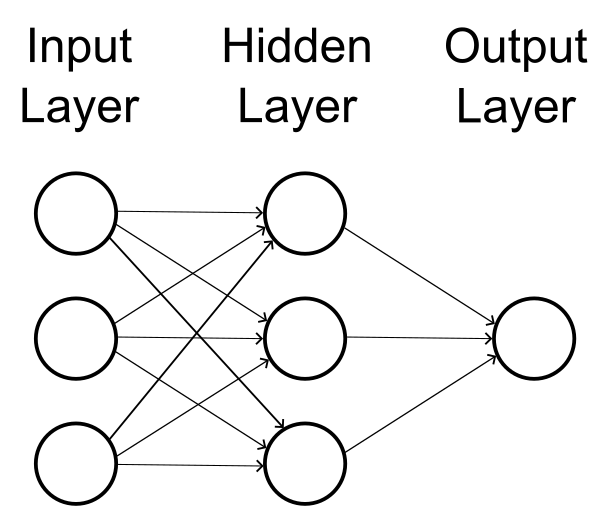
\includegraphics[width=0.5\textwidth]{images/neural-network.png}
    \centering
    \caption{A diagram portraying the structure of a simple three layer \gls{mlp}.}
    \label{fig:nn}
\end{figure}

The training of an \gls{ann} consists of the initial assignment of random weights to each of the neurons connections followed by an iterative minimization of the sum of squared errors over all of the training data. This process is carried out via a learning algorithm. The most commonly used are:
\begin{itemize}
    \item \Gls{sbp} which is a steepest gradient descent algorithm. For \gls{sbp} the weight $\omega_{j}$ in iteration $n$ is updated via the following equation:

$\Delta\omega_{j}(n) = -\eta\frac{\partial E}{\partial \omega_{j}}+\alpha\Delta\omega_{j}(n-1)$

    where:
        \begin{itemize}
            \item $\omega_{j}$ are the connection weights.
            \item $eta$ is the learning rate.
            \item $E$ is the sum of squared error.
            \item $alpha$ is the momentum factor.
            \item $n$ is the iteration.
        \end{itemize}

    \item \Gls{scg} is a method that searches along conjugate directions in successive iterations for faster convergence. Selection of search direction is governed by the following equations:

        $\omega_{k+1} = \omega_{k} + \alpha_{k}p_{k}$ \\
        $p_{k} = -E'(\omega) + \alpha_{k}p_{k+1}$

        where:
        \begin{itemize}
            \item $\omega_{k+1}, \omega_{k}$ are the connection weights.
            \item $\alpha$ is the momentum factor.
            \item $p_{k}, p_{k+1}$ are the conjugate directions in successive iterations.
            \item $E$ is the sum of squared error.
        \end{itemize}

    \item \Gls{bpr} is an extension of the \gls{sbp} algorithm which constrains network parameters via regularization. A modification is made to the loss function:

        $F = \gamma E + \frac{1 - \gamma}{n} \sum_{j=1}^{n}\omega_{j}^2$

        where:
        \begin{itemize}
            \item $F$ is the loss function.
            \item $\gamma$ is the performance ratio parameter.
            \item $E$ is the sum squared error.
            \item $\omega_{j}$ are the connection weights.
            \item $n$ is the iteration.
        \end{itemize}
\end{itemize}

\subsubsection{Support vector machine}\label{Support vector machine}

The \glsxtrlong{svm} is a model designed for the supervised classification of labeled data belonging to two classes \cite{vapnik-svm}. It enables the discovery of an optimal line or hyperplane that maximizes the distance between each class in an N-dimensional space. An example of its application for a 2-dimensional space can be seen in figure \ref{fig:svm}. \gls{svm} can handle the linear separation of data as well as the non-linear separation of data via a kernel trick \cite{non-linear-svm}. The most popular non-linear kernels are the: polynomial kernel, \gls{rbf} and sigmoid kernel \cite{ibm-svm}. An extension of the original hard-margin \gls{svm} is the soft-margin \gls{svm}. The difference between them is that with the hard-margin \gls{svm} data points will be perfectly separated outside of the support vectors while soft-margin classification will allow some misclassification through the use of a slack variable \cite{vapnik-svm}.
The hard-margin \gls{svm} is defined as:\\

    $\underset{w, b}{minimize}\quad \frac{1}{2}\left\| \omega \right\|^2$

    $subject\ to\quad y_{i}(\omega^Tx_{i}-b) \ge 1\quad \forall i \in \{1,...,n\}$ \\

    where:
    \begin{itemize}
        \item $\omega$ is the normal vector to the hyperplane.
        \item $b$ is the distance of the hyperplane from the origin.
        \item $y_{i}$ is the class label for each training instance.
        \item $x_{i}$ is the feature vector for each training instance.
        \item $n$ is the total number of training instances.
    \end{itemize}

While the soft-margin \gls{svm} is defined as:\\

    $\underset{w, b, \zeta}{minimize}\quad \left\| w \right\|^2 + C\sum_{i=1}^{n}\zeta_{i}$

    $subject\ to\quad y_{i}(w^Tx_{i}-b) \ge 1 - \zeta_{i}$ \\

    where:
    \begin{itemize}
        \item $\omega$ is the normal vector to the hyperplane.
        \item $b$ is the distance of the hyperplane from the origin.
        \item $y_{i}$ is the class label for each training instance.
        \item $x_{i}$ is the feature vector for each training instance.
        \item $n$ is the total number of training instances.
        \item $C$ is the regularization parameter.
        \item $\zeta_{i}$ are the slack variables.
    \end{itemize}

Another extension of the \glsxtrshort{svm} is \gls{svr} which enables the application of \glsxtrshort{svm} to regression problems \cite{vapnik-svr,svr}.

\gls{svr} is defined as:\\

    $minimize\quad \frac{1}{2} \left\| w \right\|^2$

    $subject\ to\quad \left| y_{i} - \langle w,x_{i} \rangle - b \right| \le \varepsilon$\\

    where:
    \begin{itemize}
        \item $\omega$ is the normal vector to the hyperplane.
        \item $b$ is the distance of the hyperplane from the origin.
        \item $y_{i}$ is the class label for each training instance.
        \item $x_{i}$ is the feature vector for each training instance.
        \item $n$ is the total number of training instances.
        \item $\varepsilon$ is the band of tolerance.
    \end{itemize}

\begin{figure}
    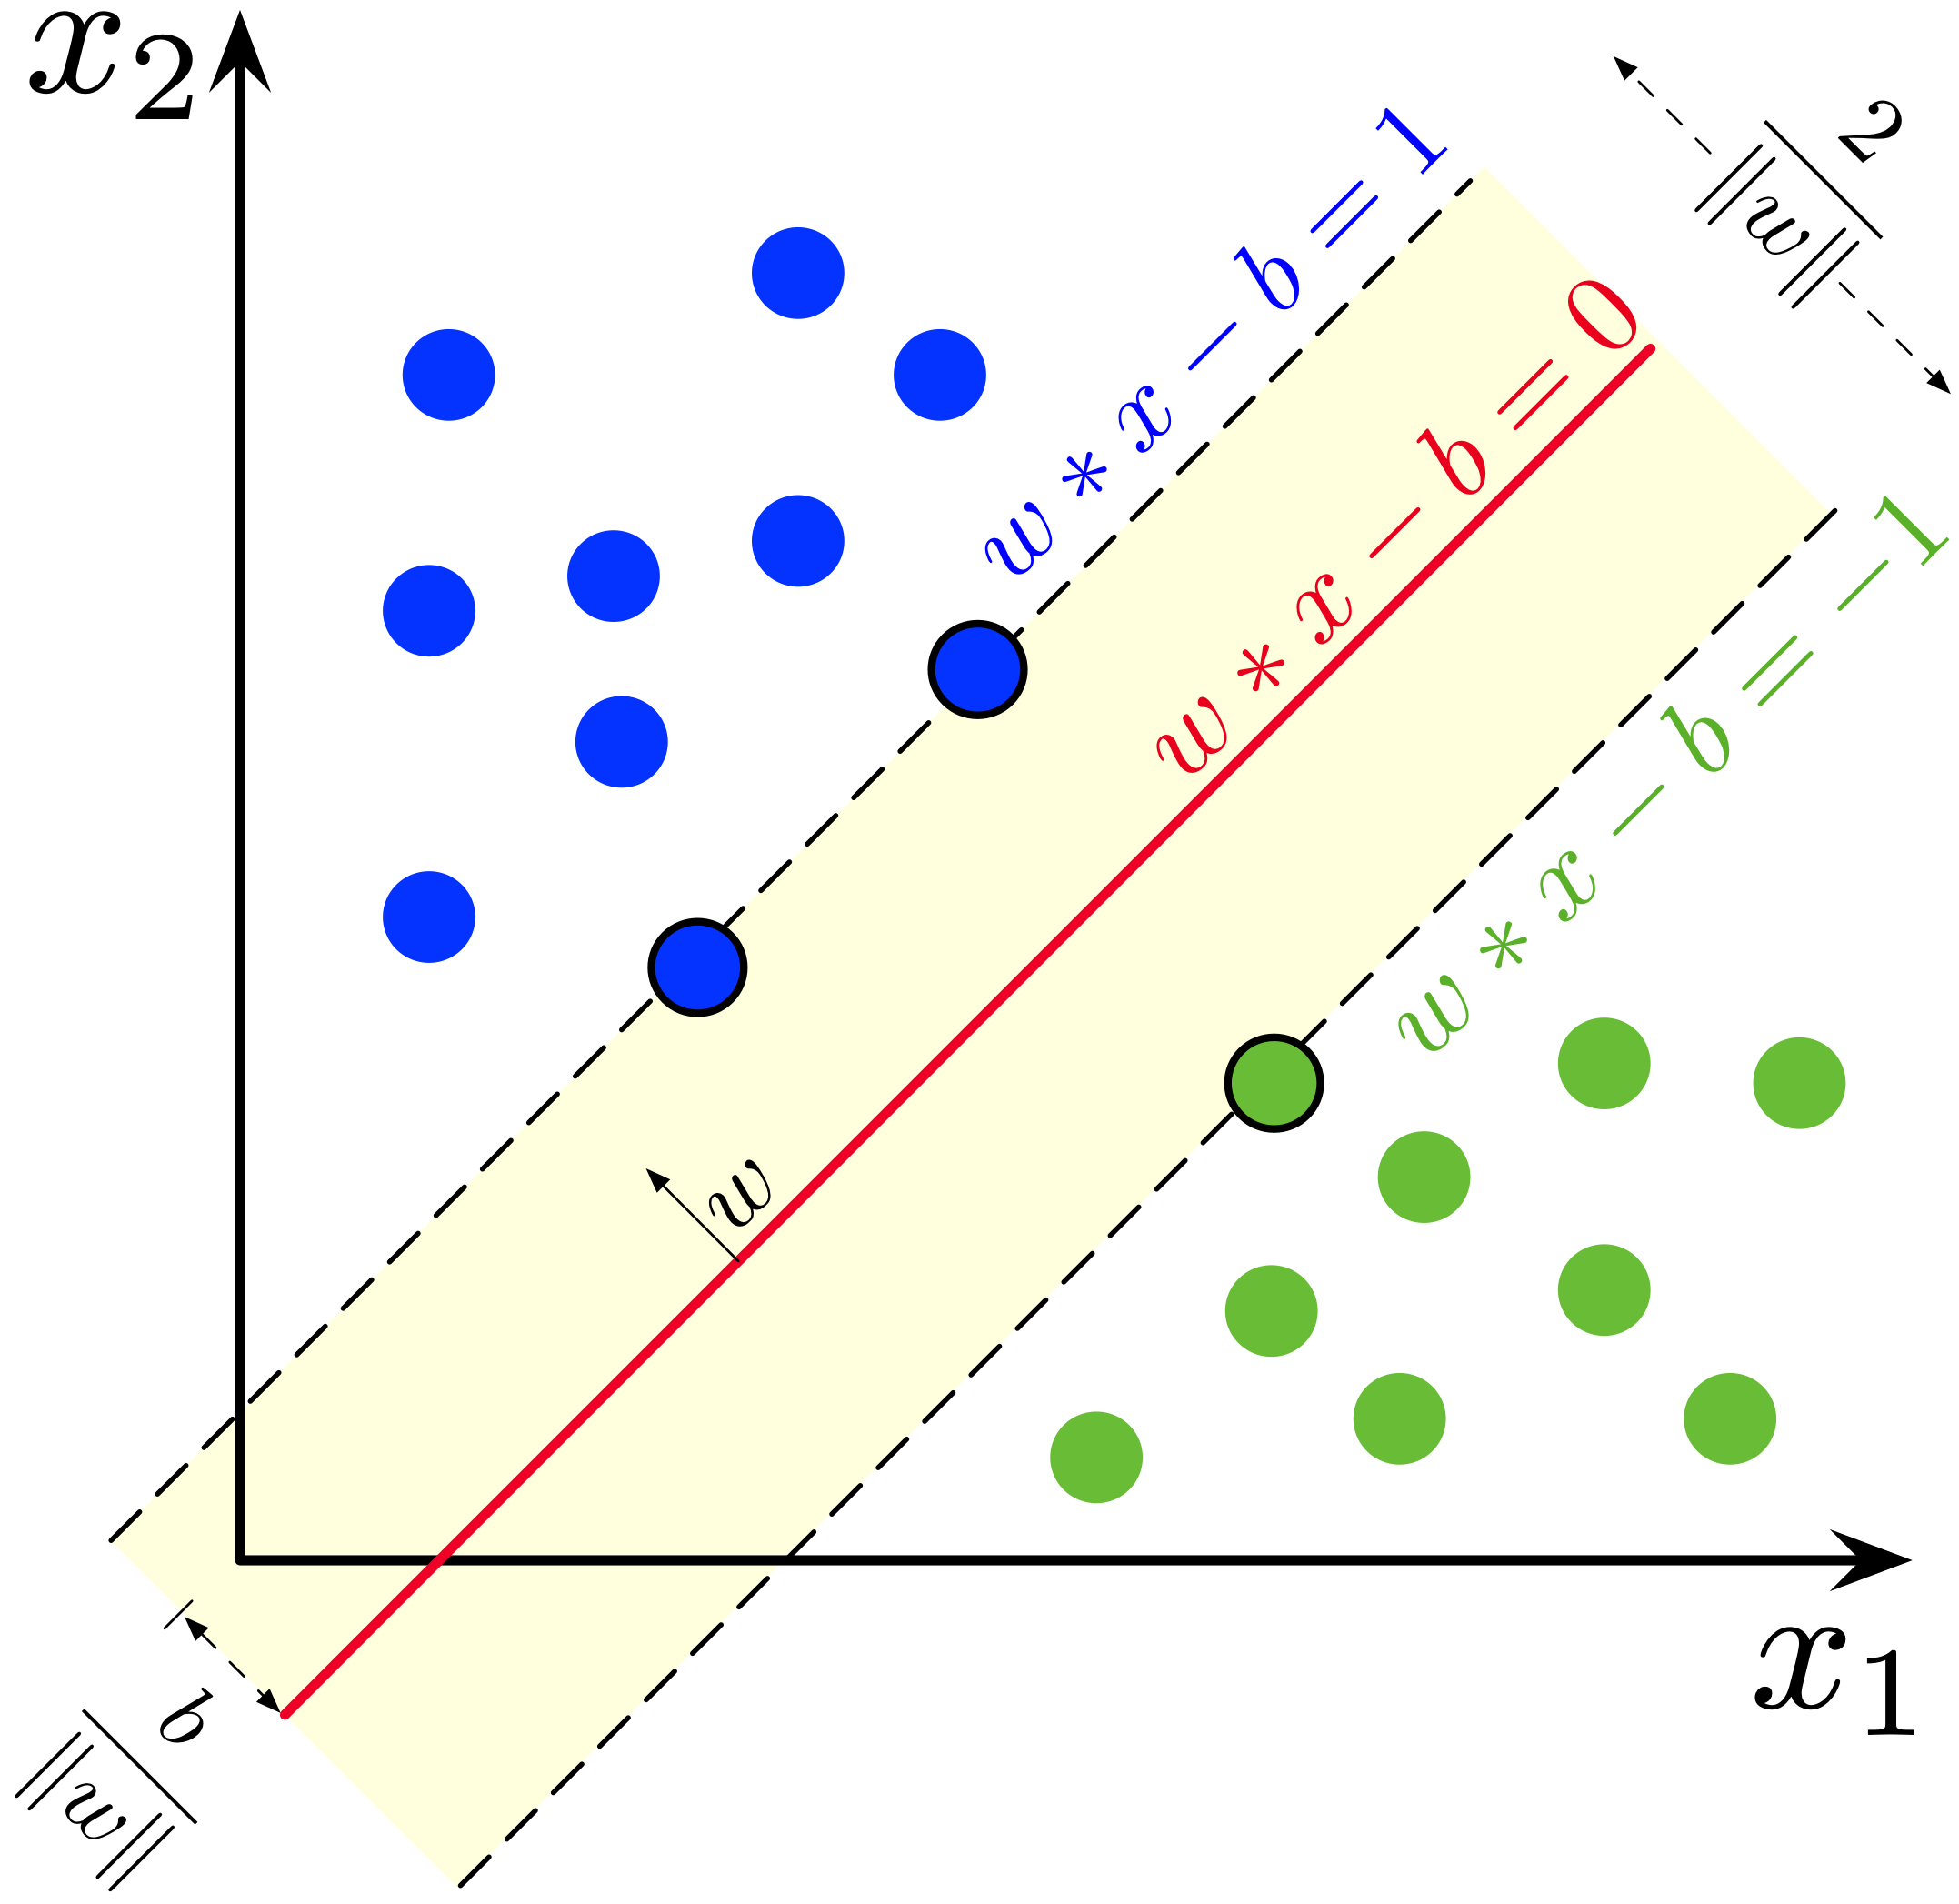
\includegraphics[width=0.5\textwidth]{images/svm-margin.png}
    \centering
    \caption{Maximum-margin hyperplane and margin for an \gls{svm} trained on two classes \cite{svm-margin}.}
    \label{fig:svm}
\end{figure}

The primary tunable parameters of a \glsxtrshort{svm} are \cite{scikit-svr,svr}:
\begin{itemize}
    \item Kernel function - determines the type of decision boundary. 
    \item Kernel hyperparameters - degree ($d$) for the polynomial kernel, gamma ($\gamma$) for the \glsxtrshort{rbf}, polynomial and sigmoid kernels and Gamma ($\gamma$) and intercept ($r$) for the polynomial and sigmoid kernels.
    \item Regularization strength ($C$) - controls the trade-off between maximizing the margin and minimizing the training error.
    \item Loss function - hinge loss for \glsxtrshort{svm} classification and $\varepsilon$-insensitive loss for \glsxtrshort{svr}.
    \item Epsilon-insensitive margin ($\varepsilon$) - margin of tolerance where no penalty is associated in the training loss function.
\end{itemize}

\subsubsection{Decision tree}\label{Decision tree}

\Glspl{dt} are a non-parametric supervised learning algorithm which is used for both classification and regression tasks. They have a hierarchical recursive partitioning structure which consists of a root node, branches, internal nodes and leaf nodes. The advantages of \glsxtrlong{dt} are that they are easy to interpret, require little to no data preparation and are robust to outliers. Their disadvantages are that they are prone to overfitting, susceptible to large structural changes caused by small variations in the data and more costly than other similar techniques. Their learning strategy involves searching for optimal dataset splits using information gain or entropy based splitting criteria including the Gini impurity or Shannon entropy measures \cite{prediction,ibm-dt}.

\subsubsection{Random forest}\label{Random forest}

\Glsxtrlongpl{rf} are an instance of ensemble learning techniques. Ensemble learning involves the aggregate use of more than one model in order to produce better results \cite{ibm-ensemble}. The base unit of a \glsxtrlong{rf} is a \glsxtrlong{dt}. A large number of \glsxtrlongpl{dt} is trained and evaluated on different subsets of the data obtained from different splits of the training set. Initial randomization is done via bootstrap samples drawn from the training set with replacement. Further randomization is then added via feature bagging which selects random subsets of features. The final output of the model is the majority vote or average of the outputs of all the trees. The biggest advantages of \glsxtrlong{rf} are a reduced risk of overfitting and the easy determination of feature importance. Their greatest disadvantages are a more resource intensive and time consuming process of model training due to the use of multiple models and greater model complexity \cite{prediction, ibm-rf}.

The primary tunable parameters of a \glsxtrlong{rf} are \cite{prediction,ibm-rf}:
\begin{itemize}
    \item The number of trees.
    \item The maximum number of features to consider at each split.
    \item Splitting criterion - based on impurity measures such as Shannon Entropy or Gini impurity.
\end{itemize}

\subsection{The foreign exchange market}\label{The foreign exchange market}

The \gls{forex} market is the largest liquid financial market in the world. It is a global \gls{otc} market (there is no central market place or exchange) closest to the ideal of perfect competition. It operates 24 hours a day 5 days a week and allows banks, businesses, investment firms, hedge funds, retail traders and individuals to buy, sell and exchange currencies \cite{forex}.

\subsection{Exchange rate prediction}\label{Exchange rate prediction}

Since the fall of the Bretton Woods system of fixed exchange rates in 1976 and the establishment of floating exchange rates with the Jamaica Accords, the need for accurate forecasting of exchange rates has become increasingly important. The primary reason for this is the need for effective risk management. Knowing whether the value of a currency will rise or fall ahead of time allows not only for the mitigation of adverse currency movements, but also for well-timed and potentially highly profitable investment decisions \cite{lstm-mlp-rf,deep-learning}.

According to the \gls{emh} \cite{efficient-market-hypothesis} financial markets are efficient and their prices reflect all information available at a given point in time. An implication of this is the inability to predict future prices on the basis of historical values. As such proponents argue that market prices follow a \gls{rw} where price movements are random and independent from one another. However this hypothesis is highly contested and numerous papers have shown that currency markets exhibit inefficiencies resulting in a delay between information availability and price adjustment \cite{adaptive-markets,event-study-analysis}.

Unfortunately, even so exchange rates are notoriously difficult to predict and rarely outperform a \gls{rw} model. They exhibit a complex non-linear nature that is dependant on a wide range of variables including macroeconomic and microeconomic factors \cite{factors}.  As such there is no single model that performs well for all combinations of predictors, forecast horizons, sample periods, forecasting evaluation methods and exchange rates. At short horizons (days, weeks, months) the fluctuations of the exchange rates are significantly greater and harder to predict. At longer horizons (years) various models have been proven to be able to make predictions better than the \gls{rw} \cite{predictability}.

Given the challenges in forecasting exchange rates using traditional econometric models, in recent years researchers have increasingly turned to the application of \gls{ai} algorithms as a potential solution.

